\Question{
\lr{GSM}
}{
پارامترهای توانی در شبکه‌های
\lr{GSM}
\SubQuestion{\lr{RxLev}}
{
	این پارامتر در شبکه‌های
	\lr{GSM}
	 نشان‌دهنده‌ی توان دریافتی و واحد آن 
	\lr{dBm}
	است. معمولا یک مقدار نیز برای حداقل توان دریافتی قابل قبول در هر سلول مشخص می‌شود. البته مقادیر مختلف این پارامتر به اعداد ۰ تا ۶۳ بر اساس 
	\autoref{fig:rxlev}
	 نگاشت می‌شود.
	\begin{figure}[H]
		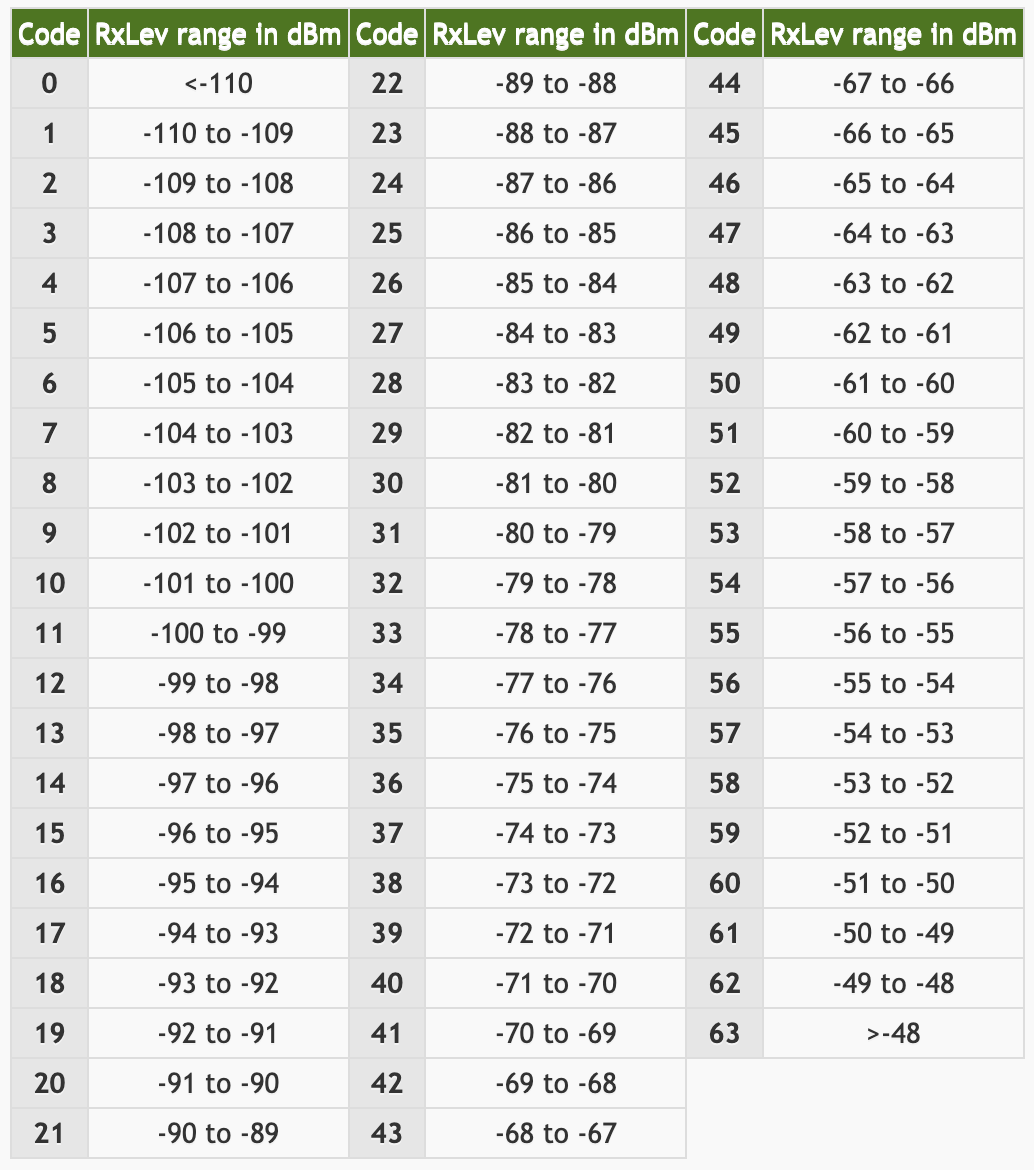
\includegraphics[width=0.85\columnwidth]{Images/rxlev.png}
		\centering
		\caption{نگاشت مقادیر مختلف
			\lr{RxLev}}
		\label{fig:rxlev}
	\end{figure}
}
\SubQuestion{\lr{RSSI}}
{
	پارامتر 
	\lr{RSSI}\LTRfootnote{Received signal strength indication}
	در شبکه‌های
	\lr{GSM}
	نشان‌دهنده‌ی توان دریافتی ناشی از تمام سیگنال‌های مرجع موجود در سلول سرویس‌دهنده و سلول‌های همسایه و نویز در کل پهنای باند حامل فرکانسی است و واحد آن 
	\lr{dBm}
	است. تفاوت آن با 
	\lr{RxLev}
	این است که 
	\lr{RSSI}
	یک پارامتر درونی و داخل 
	\lr{chipset}
	است. این پارامتر مقادیر منفی دارد و هر چقدر که به صفر نزدیک‌تر باشد، سیگنال قوی‌تر است. این پارامتر در نسل‌های بعدی شبکه‌های تلفن همراه نیز وجود دارد.
}
}